%%%%%%%% ICML 2022 EXAMPLE LATEX SUBMISSION FILE %%%%%%%%%%%%%%%%%

\documentclass[nohyperref]{article}

% Recommended, but optional, packages for figures and better typesetting:
\usepackage{microtype}
\usepackage{graphicx}
\usepackage{bbm}
\usepackage{subfigure}
\usepackage{booktabs} % for professional tables

% hyperref makes hyperlinks in the resulting PDF.
% If your build breaks (sometimes temporarily if a hyperlink spans a page)
% please comment out the following usepackage line and replace
% \usepackage{icml2022} with \usepackage[nohyperref]{icml2022} above.
\usepackage{hyperref}


% Attempt to make hyperref and algorithmic work together better:
\newcommand{\theHalgorithm}{\arabic{algorithm}}

% Use the following line for the initial blind version submitted for review:
\usepackage[accepted]{icml2022}

% If accepted, instead use the following line for the camera-ready submission:
% \usepackage[accepted]{icml2022}

% For theorems and such
\usepackage{amsmath}
\usepackage{amssymb}
\usepackage{mathtools}
\usepackage{amsthm}

% if you use cleveref..
\usepackage[capitalize,noabbrev]{cleveref}

%%%%%%%%%%%%%%%%%%%%%%%%%%%%%%%%
% THEOREMS
%%%%%%%%%%%%%%%%%%%%%%%%%%%%%%%%
\theoremstyle{plain}
\newtheorem{theorem}{Theorem}[section]
\newtheorem{proposition}[theorem]{Proposition}
\newtheorem{lemma}[theorem]{Lemma}
\newtheorem{corollary}[theorem]{Corollary}
\theoremstyle{definition}
\newtheorem{definition}[theorem]{Definition}
\newtheorem{assumption}[theorem]{Assumption}
\theoremstyle{remark}
\newtheorem{remark}[theorem]{Remark}

% Todonotes is useful during development; simply uncomment the next line
%    and comment out the line below the next line to turn off comments
%\usepackage[disable,textsize=tiny]{todonotes}
\usepackage[textsize=tiny]{todonotes}


% The \icmltitle you define below is probably too long as a header.
% Therefore, a short form for the running title is supplied here:
\icmltitlerunning{Exploring NeoRL: Critic-Regularized Regression with Past}

\begin{document}

\twocolumn[
\icmltitle{Exploring NeoRL: \\
           Critic-Regularized Regression with Past}
% \icmlsetsymbol{equal}{*}

\begin{icmlauthorlist}
\icmlauthor{Haotian Chu}{}
\end{icmlauthorlist}

% You may provide any keywords that you
% find helpful for describing your paper; these are used to populate
% the "keywords" metadata in the PDF but will not be shown in the document
\icmlkeywords{Machine Learning, ICML}

\vskip 0.3in
]

\begin{abstract}


Offline reinforcement learning (RL), also known as batch RL, offers the prospect of policy optimization from large pre-recorded datasets without online environment interaction. Based on NeoRL benchmark \cite{2102.00714}, we apply a novel offline RL algorithm to learn policies from stock data using a form of \textbf{c}ritic-\textbf{r}egularized \textbf{r}egression, named CRR \cite{2006.15134}. Considering the finance setting, we provide the agent not only the current observation but also historical data (thus it is called ``\textbf{CRR with Past}"), and find out that this feature is quite essential in improving the performance. What's more, we compare several variants of CRR and discuss the choice of different weight functions.

\end{abstract}

\section{Introduction}
\label{submission}

In quantitative finance, stock trading is essentially making dynamic decisions, namely to decide where to trade, at what price, and what quantity, over a highly stochastic and complex stock market. With the development of technology, traders began to cast interest in automatic methods when dealing with finance problems. Offline reinforcement learning (RL) is one of those popular options. 

In offline RL, also known as Batch RL, the environment is no longer available during training, and the agent only relies on a static dataset $D$. The data can be gathered by some unknown behavioral policy (or a mixture of policies) $\pi_\mu$. Because the data is static and the policy has no access to the environment during training, the agent is faced with the problem of extrapolation error \cite{kidambi2020morel}, as well as losing its ability to correct its estimation inaccuracies.

The naive application of off-policy RL algorithms with function approximation to the offline setting has often failed, and a shared conclusion is that failure comes from overly optimistic Q-estimates, as well as inappropriate extrapolation beyond the observed data. 

In this paper, we choose \textbf{c}ritic-\textbf{r}egularized \textbf{r}egression \cite{2006.15134} algorithm to learn policies from data. CRR essentially reduces offline policy optimization to a form of value-filtered regression that requires minimal algorithmic changes to standard actor-critic methods.

In the experiment, we rely heavily on the user interface and results of NeoRL \cite{2102.00714}, a suite of near real-world benchmarks for offline RL. Beyond the finance setting, NeoRL includes robotics, industrial control, and city management tasks with real-world nature. Currently, NeoRL provides different sizes from low to high amounts, and different quality of data collected from corresponding simulators, and benchmark recently proposed model-free and model-based offline RL methods as a reference. The online and offline evaluations are both performed for selecting the hyper-parameters for each algorithm.

After exploring the finance dataset of NeoRL, we find that the observation vector is merely a snapshot of daily stock market. Although it makes sense in the setting of reinforcement learning, it seems to contradict to the logic of finance, where traders usually make the decision of purchase (selling) after analyzing the historical data for a long time. 

As a result, we derive \textbf{``CRR with Past"}. considering the sequential logic of stock data, we concatenate the past $t$ days' prices information to the observation vector, providing the agent the observation within a period of time instead of a simple snapshot. 

What's more, our experiments discuss several variants of CRR model and show that they outperforms several state-of-the-art offline RL algorithms by a significant margin.

\section{Momentum Indicators}


Considering the finance setting of the environment, we will introduce some economic analyzing techniques to help make investment decisions\cite{2011.09607}. 

\textbf{MACD.} Developed by Gerald Appel, the Moving Average Convergence Divergence oscillator (MACD) is one of the simplest and most effective momentum indicators available. The MACD turns two trend-following indicators into a momentum oscillator by subtracting the longer moving average from the shorter moving average. Because the MACD is unbounded, it is not particularly useful for identifying overbought and oversold levels. 

\textbf{RSI.} Relative Strength Index (RSI) is another momentum indicator used in technical analysis that measures the magnitude of recent price changes to evaluate overbought or oversold conditions in the price of a stock or other asset. The RSI is displayed as an oscillator (a line graph that moves between two extremes) and can have a reading from 0 to 100. The indicator was originally developed by J. Welles Wilder Jr. and introduced in his seminal 1978 book, “New Concepts in Technical Trading Systems.”


\textbf{CCI.} The Commodity Channel Index (CCI) is a momentum-based oscillator used to help determine when an investment vehicle is reaching a condition of being overbought or oversold. Developed by Donald Lambert, this technical indicator assesses price trend direction and strength, allowing traders to determine if they want to enter or exit a trade, refrain from taking a trade, or add to an existing position. In this way, the indicator can be used to provide trade signals when it acts in a certain way.

All the three indicators are included in the observation vector as shown in Fig. \ref{nor}. 

\begin{figure}[H]
\begin{center}
\vspace*{-3mm}
\centerline{
\includegraphics[width=\columnwidth]{nor.png}}
\vspace*{-3mm}
\caption{The Observation Vector is a concatenation of the current balance, prices, MACD, RSI and CCI of the total 30 stocks.}
\vspace*{-3mm}
\label{nor}
\end{center}
% \vskip -0.2in
\end{figure}




\section{Critic Regularized Regression}

Critic Regularized Regression (CRR), is a simple, yet effective, method for offline RL.

\subsection{Policy Learning with CRR}

Firstly, consider the policy evaluation in the setting of offline RL. Suppose we are given a fixed dataset $\mathcal{B}$ containing either individual transition tuples $(s_t, a_t, r_t, s_{t+1})$. An important step in many off-policy learning approaches is off-policy policy evaluation. This often involves learning an approximation to the Q-function minimizing a temporal difference loss similar to the following
\begin{equation}\label{eq1}
    \mathbb{E}_{\mathcal{B}}\Big[D\big(Q_\theta(s_t, a_t), (r_t+\gamma\mathbb{E}_{a\sim\pi(s_{t+1})}Q_{\theta'}(s_{t+1}, a))\big)\Big]
\end{equation}
where the expectation over data is approximated by sampling $(s_t, a_t, r_t, s_{t+1})\sim\mathcal{B}$ and $D$ is some divergence measure; measuring discrepancy between the current estimate of the action-value $Q_\theta(s_t, a_t)$ (for policy $\pi$) and the td-update, based on a target network \cite{mnih2015human}. We note that we make use of a distributional Q-function as in Barth-Maron et al. \cite{barth2018distributed}, instead of using a squared error for $D$.

As discussed in recent work \cite{fujimoto2019off}, due to lack of environment interaction while evaluating the value of the next state $s_{t+1}$ by $\mathbb{E}_{a\sim\pi(s_{t+1})}Q_{\theta'}(s_{t+1}, a)$, this loss may be problematic. If trained with standard RL, a parametric $\pi(\cdot|s_{t+1})$ is likely to extrapolate beyond the training data and to propose actions that are not contained in $\mathcal{B}$. For these actions $Q$ will not have been trained and may produce bad estimates.

To mitigate the problem, we should avoid evaluating $Q$ for $(s, a)\notin\mathcal{B}$. Thus, we aim to train $\pi$ by discouraging it from taking actions that are outside the training distribution. Such a requirement would be hard to achieve with standard policy gradients \cite{silver2014deterministic}. We thus change our objective to match the state-action mapping contained in the training data-but filtered by the Q-function. Specifically, we optimize
\begin{equation}\label{eq2}
    \arg\max_\pi \mathbb{E}_{(s,a)\sim\mathcal{B}}\Big[f(Q_\theta, \pi, s, a)\log\pi(a|s)\Big]
\end{equation}
where $f$ is a non-negative, scalar, function whose value is monotonically increasing in $Q_\theta$. Fundamentally, Eq. (\ref{eq2}) tries to copy actions that exist in the data, thereby restricting $\pi$. Further properties of the learning objective can be controlled through different choices of $f$, for example when $f$ := 1, Eq. (\ref{eq2}) is equivalent to Behavioral Cloning (BC). The success of BC is, however, highly dependent on the quality of the dataset $\mathcal{B}$. When $\mathcal{B}$ does not contain enough transitions generated by a policy performing well on the task, or the fraction of poor data is too large, then BC is likely to fail.


\begin{algorithm}[H]
   \caption{Critic Regularized Regression}
   \label{alg1}
\begin{algorithmic}
  \STATE {\bfseries Input:} Dataset $\mathcal{B}$, critic net $Q_\theta$, actor net $\pi_\phi$, target actor and critic nets: $\pi_{\phi'}$, $Q_{\theta'}$, function $f$
  \FOR{$n_{updates}$}
   \STATE Sample $(s_t^i, a_t^i, r_t^i, s_{t+1}^i)_{i=1}^b$ from $\mathcal{B}$.
   \STATE Update actor (policy) with gradient: \\$\qquad\nabla_\phi-\frac{1}{b}\sum_i\log\pi_\phi(a_t^i|s_t^i)f(Q_\theta, \pi_\phi, s_t^i, a_t^i)$
   \STATE Update critic with gradient: \\$\nabla_\theta\frac{1}{b}\sum_iD[Q_\theta(s_t^i, a_t^i), (r_t^i+\gamma\mathbb{E}_{a\sim\pi_{\theta'}}Q_{\theta'}(s_{t+1}^i, a))]$
   \STATE Update the target actor/critic nets every $N$ steps by copying parameters: $\theta'\leftarrow\theta, \phi'\leftarrow\phi$.
   \ENDFOR
\end{algorithmic}
\end{algorithm}



\subsection{Advantage Estimators} 

Provided $Q$ is sufficiently accurate for $(s, a)\in\mathcal{B}$ (e.g. learned using Eq. (\ref{eq1})), we can consider additional choices of $f$ that enable off-policy learning to overcome this problem:
\begin{gather}
    f:=\mathbbm{1}[\hat{A}_\theta(s, a)>0]\label{eq3}\\f:=\exp\big(\hat{A}_\theta(s, a)/\beta\big)\label{eq4}
\end{gather}
where $\beta>0$ is a hyper-parameter, $\mathbbm{1}$ the indicator function, and $\hat{A}_\theta(s, a)$ is an estimated advantage function. Intuitively, Eq. (\ref{eq3}) entails BC on a filtered dataset where the filtering increases the average quality of the actions we learn from. The filter is defined in terms of the value of the current policy. For each $f$, we should further consider different advantage estimators:

\begin{gather}
    \hat{A}_{mean}(s_t, a_t)=Q_\theta(s_t, a_t)-\frac{1}{m}\sum_{j=1}^mQ_\theta(s_t, a^j)\label{eq5}\\\hat{A}_{max}(s_t, a_t)=Q_\theta(s_t, a_t)-\max_{j=1}^mQ_\theta(s_t, a^j)\label{eq6}
\end{gather}

In the beginning, we intended to simply consider $\hat{A}_{mean}$, but according to the original paper of CRR \cite{2006.15134}, for small $m$, $\hat{A}_{mean}$ may overestimate the advantage due to stochasticity. We therefore also consider $\hat{A}_{max}$, a pessimistic estimate of the advantage. 

As we have two choices of weight functions and two different types of advantage estimators, we can derive four variants of CRR algorithm. In Table \ref{raw table}, we have made the comparison of four variants.


\begin{table}[H]
\caption{The online evaluation results trained on \textbf{raw data}. Policies are measured by their episode return and averaged over 100 episodes.}
\label{raw table}
\vskip 0.15in
\begin{center}
\begin{small}
\begin{sc}
\begin{tabular}{lcccr}
\toprule
variants & high-100 & medium-100 & low-100 \\
\midrule
mean-exp & 356 & 315 & 328\\
mean-binary & 229 & 251 & 174\\
max-exp & \textbf{380} & \textbf{332} & 335\\
max-binary & 308 & 170 & \textbf{438}\\
\bottomrule
\end{tabular}
\end{sc}
\end{small}
\end{center}
\vskip -0.1in
\end{table}

``MEAN" corresponds to Eq. (\ref{eq5}) and ``MAX" is Eq. (\ref{eq6}), while ``BINARY" corresponds to Eq. (\ref{eq3}) and ``EXP" corresponds to Eq. (\ref{eq4}). ``HIGH-100" represents the dataset ``finance-high-100" of NeoRL \cite{2102.00714}.

From the table, we can roughly reach a conlcusion that the pessimistic estimator $\hat{A}_{max}$ performs better than $\hat{A}_{mean}$, but the difference of weight functions is still subtle. In the following section, we will gain insight into Eq. (\ref{eq4}).


\subsection{Exponential Weighting} 

We can gain insight into Eq. (\ref{eq4}) by realizing that it approximately implements a regularized policy improvement step in a policy iteration scheme. Consider
\begin{equation}
    \mathcal{L}(q, \mu_{\mathcal{B}})=\mathbb{E}_{s\sim\mathcal{B}}\Big[\mathbb{E}_q[Q_\theta(s, a)]+\beta\text{KL}[q(\cdot|s), \mu_\mathcal{B}(\cdot|s)]\Big]
\end{equation}
where $\mu_\mathcal{B}$ is the policy that generated the data, and $q(a|s)\propto\exp(\hat{A}_\theta(s, a)/\beta)$. By minimizing the cross-entropy $H[q(\cdot|s), \pi_\phi(\cdot|s)]$, we can project this distribution back onto the parametric policy $\pi_\phi$. In Fig. \ref{beta nor}, we plot the average reward of different $\beta$. When trained on medium quality, the best performance take place when $\beta$ equals to 4. It should be noted that, as $\beta\to\infty$, this objective becomes behavior cloning (BC). 

\begin{figure}[H]
\begin{center}
\vspace*{-3mm}
\centerline{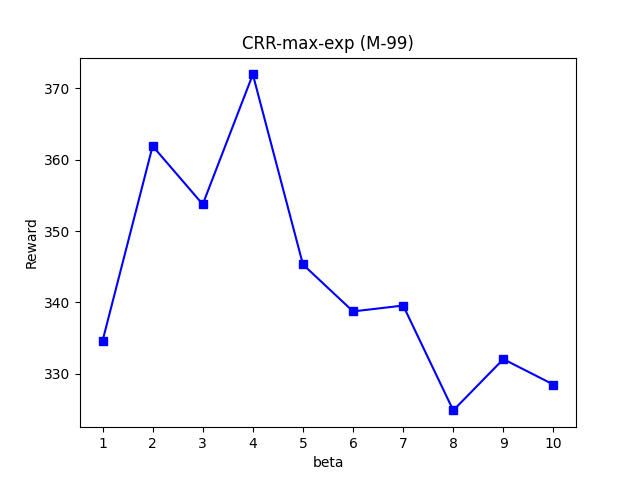
\includegraphics[width=\columnwidth, clip]{beta normal.png}}
\caption{Reward of different $\beta$.}
\vspace*{-3mm}
\label{beta nor}
\end{center}
\end{figure}


\section{The effect of past information}


In the setting of reinforce learning, the input of the model is usually a snapshot of the environment, which is commonly accepted in various RL frameworks. However, in some downstream tasks, ``memory'' (historical data) is important during decision making, and stock trading is a definitely one of them.

In reality, traders usually make the decision of purchase (selling) after analyzing the historical data for a long time. Some trading strategies even rely on historical data to conclude the market trend.

As a result, instead of simply feeding raw data into CRR model, we concatenate the past $t$ days' prices information to the observation vector (Fig. \ref{past}), enabling the agent to take the past into consideration while making decision. 


\begin{figure}[H]
\begin{center}
\centerline{
\includegraphics[width=\columnwidth]{past.png}}
\vspace*{-3mm}
\caption{The information of past $t$ days' prices is concatenated to the observation vector.}
\label{past}
\end{center}
\end{figure}


To test the effect of historical information, we compare the performance when models are trained on raw data and data with past information. And the result is plotted as follows. (The remains are in the Appendix.) 
\begin{figure}[H]
\begin{center}
\vspace*{-3mm}
\centerline{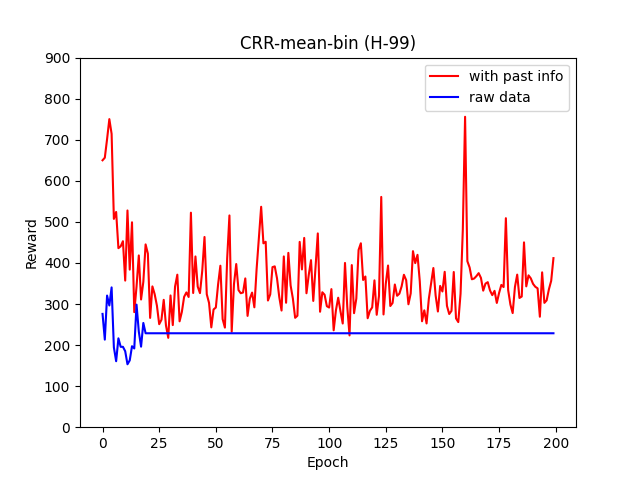
\includegraphics[width=\columnwidth, clip]{CRR-mean-bin (H-99).png}}
\centerline{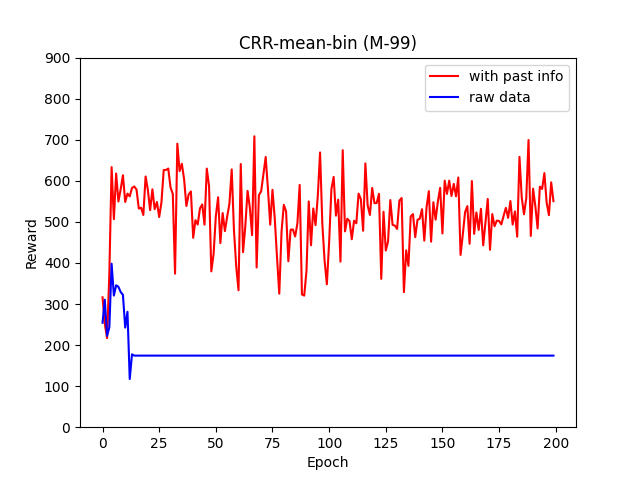
\includegraphics[width=\columnwidth, clip]{CRR-mean-bin (M-99).png}}
\centerline{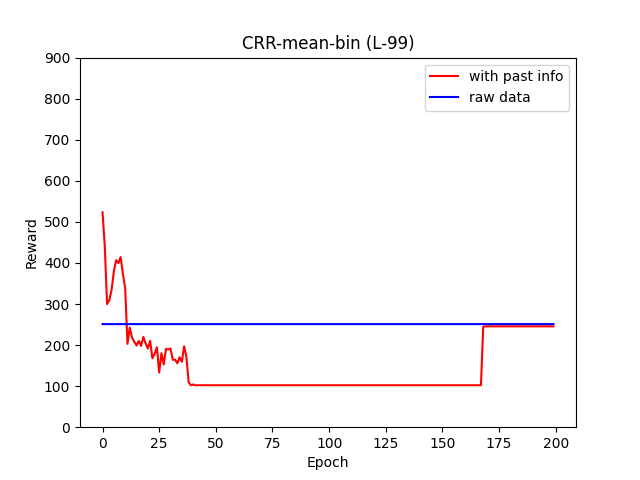
\includegraphics[width=\columnwidth, clip]{CRR-mean-bin (L-99).png}}
\caption{Reward of CRR in the first 200 epochs. In this figure, weight function is chosen according to Eq. (\ref{eq3}) and Eq. (\ref{eq5}). ``H-99'' represents ``finance-high-100" dataset of NeoRL \cite{2102.00714}.}
\vspace*{-3mm}
\label{CRR-99}
\end{center}
\end{figure}


The figure shows that CRR model trained on data with past information outperforms that trained on raw data, especially when data is of medium and high quality. 

To generalize the conclusion, we also make the comparison based on Behavioral Cloning (BC) algorithm, which is a baseline of learning method in the NeoRL benchmark.


\begin{figure}[H]
\begin{center}
\vspace*{-3mm}
\centerline{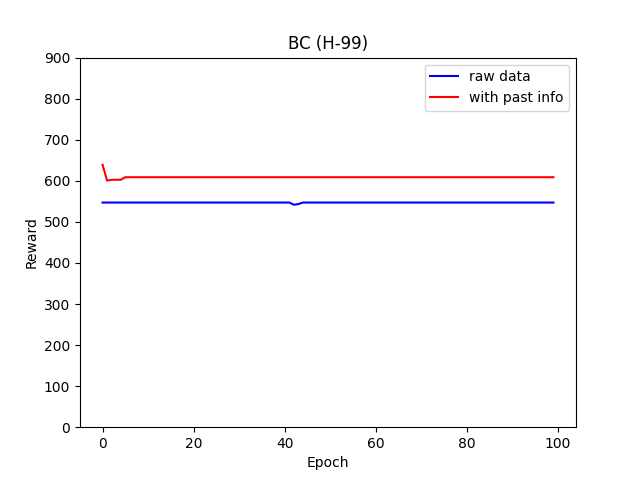
\includegraphics[width=\columnwidth, clip]{BC-H.png}}
\centerline{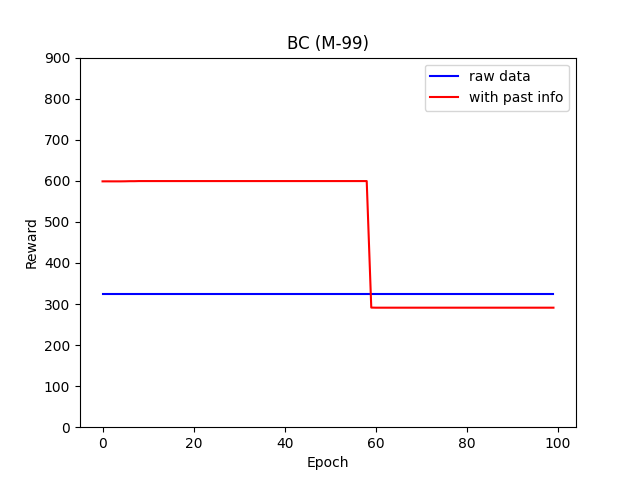
\includegraphics[width=\columnwidth, clip]{BC-M.png}}
\centerline{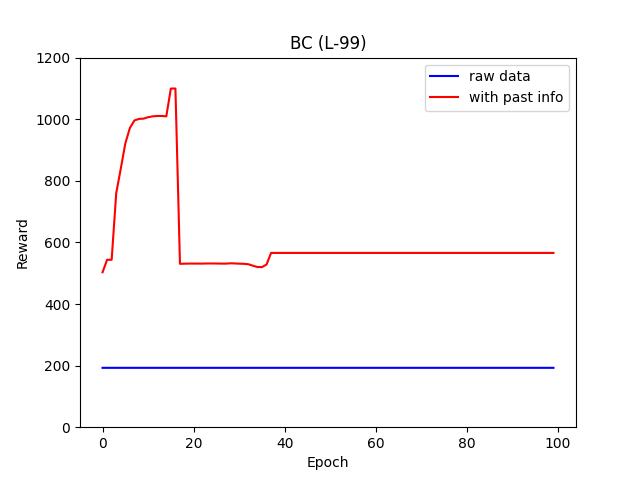
\includegraphics[width=\columnwidth, clip]{BC-L.png}}
\caption{Reward of BC in the first 200 epochs.}
\vspace*{-3mm}
\label{BC-99}
\end{center}
\end{figure}

We can conclude from the figure that training on data that contains historical information helps BC improves its performance too. It should be noticed that, learned from high-quality processed data, BC can achieve performance similar to the expert policy according to NeoRL benchmark \cite{2102.00714}.

Then, in order to test the effect of past information on CRR variants, we train four variants using processed data (Table \ref{pro table}). 


\begin{table}[H]
\caption{The online evaluation results trained on \textbf{processed data}. The number in the parenthesis stands for the difference between evaluation results trained on raw data.}
\label{pro table}
\vskip 0.15in
\begin{center}
\begin{small}
\begin{sc}
\begin{tabular}{lcccr}
\toprule
variants & high-100 & medium-100 & low-100 \\
\midrule
mean-exp & 250 (-156) & \textbf{540} (+225) & \textbf{318} (-10)\\
mean-binary & 353 (+124) & 533 (+282) & 194 (+20)\\
max-exp & 286 (-94) & 509 (+177) & 301 (-34)\\
max-binary & \textbf{378} (+70) & 458 (+288) & 176 (-262)\\
\bottomrule
\end{tabular}
\end{sc}
\end{small}
\end{center}
\vskip -0.1in
\end{table}

From the comparison with Table \ref{raw table}, we can easily find out that the performance of optimistic estimator $\hat{A}_{mean}$ grows significantly after we provide the agent with historical information, which implies that historical information might lower the probability of overestimation.


It should be noted that, interestingly, the effect of historical data is tremendously marvelous on dataset of medium quality. One possible explanation might be that, agent can already learn mature strategy from high-quality raw dataset, therefore the additional historical information can hardly further improve the result. 

At last, we plot the average reward of different $\beta$ using processed data (Fig. \ref{beta past}).

\begin{figure}[H]
\begin{center}
\vspace*{-3mm}
\centerline{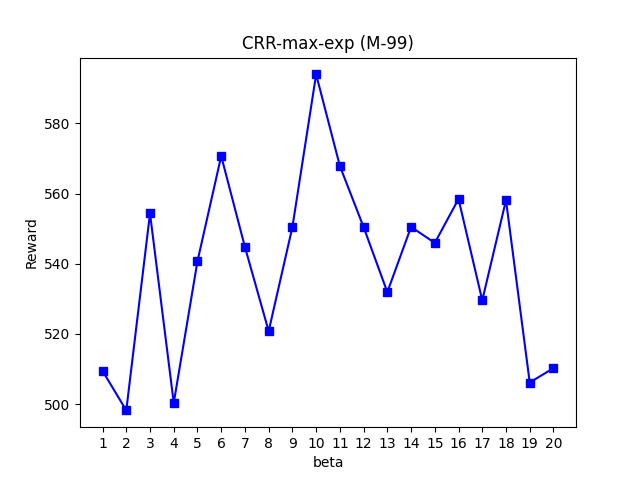
\includegraphics[width=\columnwidth, clip]{beta past.png}}
\caption{Reward of different $\beta$ when trained on processed data.}
\vspace*{-3mm}
\label{beta past}
\end{center}
\end{figure}

Different from Fig. \ref{beta nor}, when trained on data with historical information, the reduction of performance appears when $\beta>10$. (In previous experiment, the performance declines when $\beta>4$.)

\section{Conclusion}

From several simple experiments and comparison with NeoRL benchmark, we have depicted a rough picture of CRR model as well as its variants, and have provided a comprehensive discussion about the effect of historical data.

When models are trained on raw data, we find on that the pessimistic estimator $\hat{A}_{max}$ performs better than $\hat{A}_{mean}$, while the difference between binary and exponential weight function is still subtle (Table \ref{raw table}). Considering the exponential weight function, the best performance take place when $\beta$ equals to 4 (Fig. \ref{beta nor}, trained on raw data of medium quality for example), which does make sense because the model becomes behavior cloning (BC) as $\beta\to\infty$, which is a baseline learning method of NeoRL benchmark.


Although it is generally accepted that the input of RL model is a snapshot of current environment, we think that it contradicts to the logic of stock trading. Therefore, considering the finance setting, we concatenate the past $t$ days' prices information to the observation vector, and find that CRR model trained on data with past information outperforms that trained on raw data, especially when data is of medium and high quality (Fig. \ref{CRR-99}). To generalize the effect of historical information, we also test BC algorithm, and find that training on processed data helps BC improves its performance too. 

We also train four variants using processed data to futher explore the effect of past information (Table \ref{pro table}), and find out that the performance of optimistic estimator $\hat{A}_{mean}$ grows significantly after the data are processed, which implies that historical information might lower the probability of overestimation. From the comparison with previous experiment, we surprisingly discover that the effect of historical data is unbelievably marvelous on dataset of medium quality. We think it might because agent can already learn mature strategy from high-quality raw dataset, therefore the additional historical information can hardly further improve the result. What's more, when trained on data with historical information, the reduction of performance appears when $\beta>10$ (Fig. \ref{beta past}).

On the other hand, there exist some weaknesses to this work and further exploration can be done in the future. For example, the effect of historical data can be tested on algorithms of more diversity (CQL maybe, or some model-based methods), because BC is actually a special form of CRR as well. Also, although the idea of ``CRR with past" creates great performance enhancement in the finance setting, whether this improvement can be generalized to other downstream tasks remains to be explored.  


\nocite{langley00}

\bibliography{example_paper}
\bibliographystyle{icml2022}


\newpage
\appendix
\onecolumn
\section{The effect of past information}

\begin{figure}[H] 
\begin{minipage}[t]{0.5\linewidth} 
\centering 
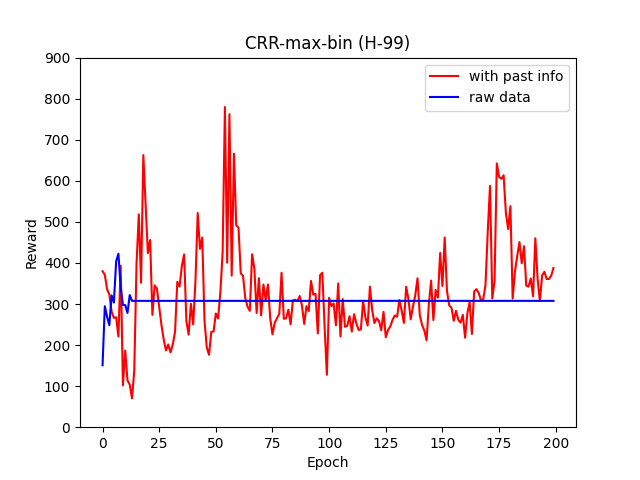
\includegraphics[width=3in]{CRR-max-bin (H-99).png}
    \caption{CRR-max-bin trained on ``finance-high-100".}
\end{minipage}
\begin{minipage}[t]{0.5\linewidth} 
\centering 
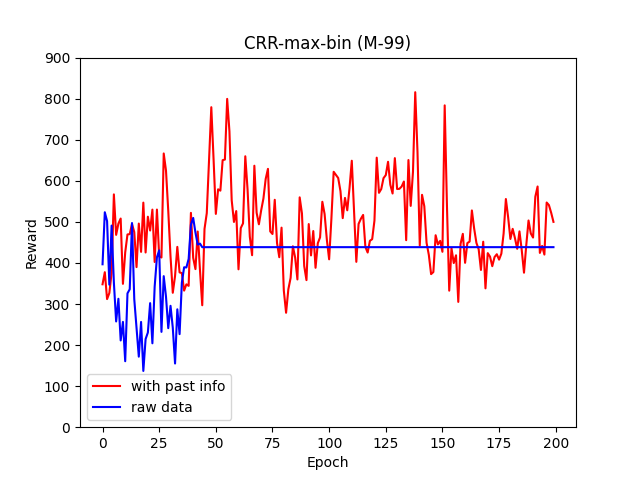
\includegraphics[width=3in]{CRR-max-bin (M-99).png}
    \caption{CRR-max-bin trained on ``finance-medium-100".}
\end{minipage} 
\end{figure}


\begin{figure}[H] 
\begin{minipage}[t]{0.5\linewidth} 
\centering 
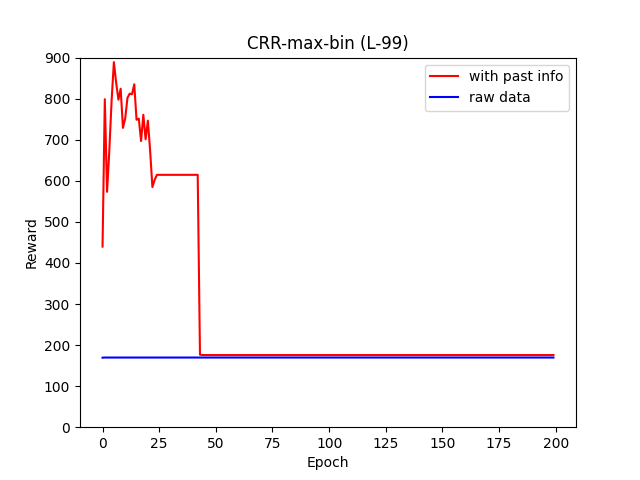
\includegraphics[width=3in]{CRR-max-bin (L-99).png}
    \caption{CRR-max-bin trained on ``finance-low-100".}
\end{minipage}
\begin{minipage}[t]{0.5\linewidth} 
\centering 
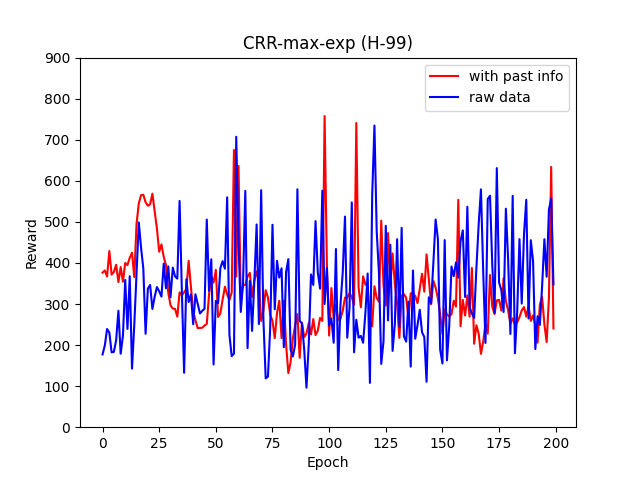
\includegraphics[width=3in]{CRR-max-exp (H-99).png}
    \caption{CRR-max-exp trained on ``finance-high-100".}
\end{minipage} 
\end{figure}


\begin{figure}[H] 
\begin{minipage}[t]{0.5\linewidth} 
\centering 
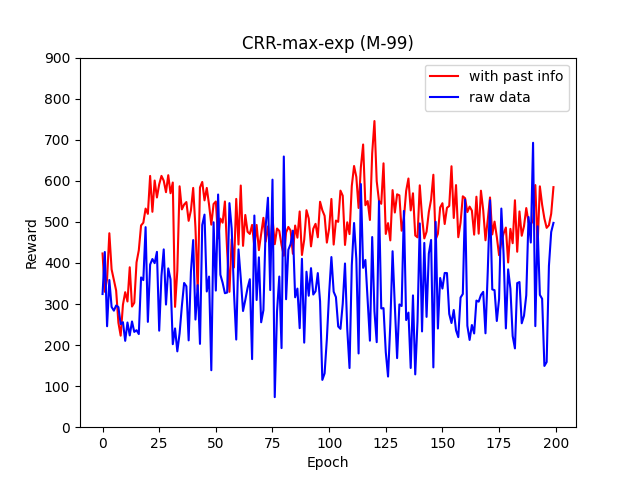
\includegraphics[width=3in]{CRR-max-exp (M-99).png}
    \caption{CRR-max-exp trained on ``finance-medium-100".}
\end{minipage}
\begin{minipage}[t]{0.5\linewidth} 
\centering 
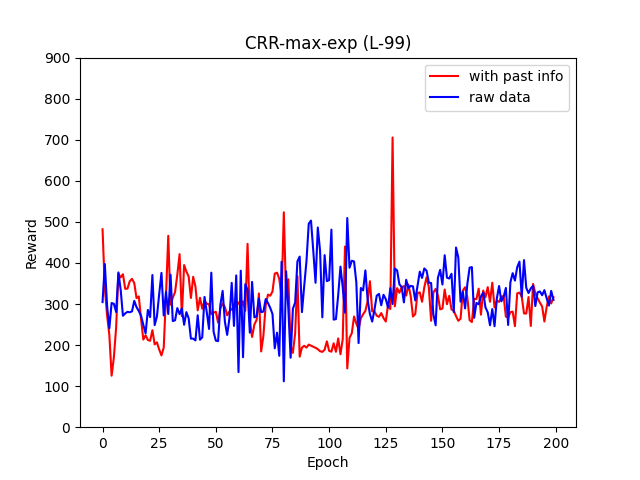
\includegraphics[width=3in]{CRR-max-exp (L-99).png}
    \caption{CRR-max-exp trained on ``finance-low-100".}
\end{minipage} 
\end{figure}



\begin{figure}[H] 
\begin{minipage}[t]{0.5\linewidth} 
\centering 
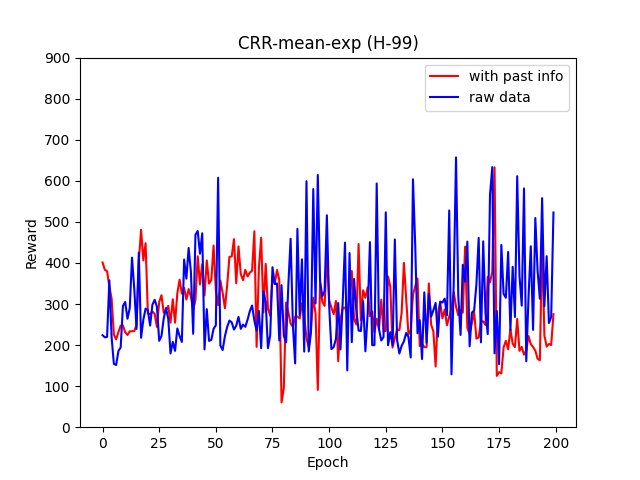
\includegraphics[width=3in]{CRR-mean-exp (H-99).png}
    \caption{CRR-mean-exp trained on ``finance-high-100".}
\end{minipage}
\begin{minipage}[t]{0.5\linewidth} 
\centering 
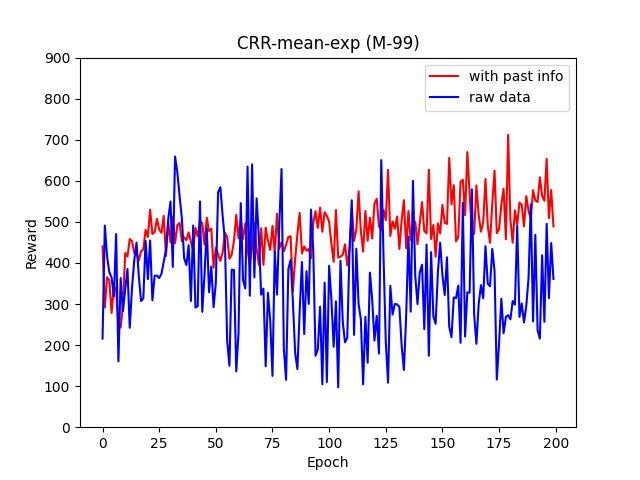
\includegraphics[width=3in]{CRR-mean-exp (M-99).png}
    \caption{CRR-mean-exp trained on ``finance-medium-100".}
\end{minipage} 
\end{figure}


\begin{figure}[H] 
\begin{minipage}[t]{0.5\linewidth} 
\centering 
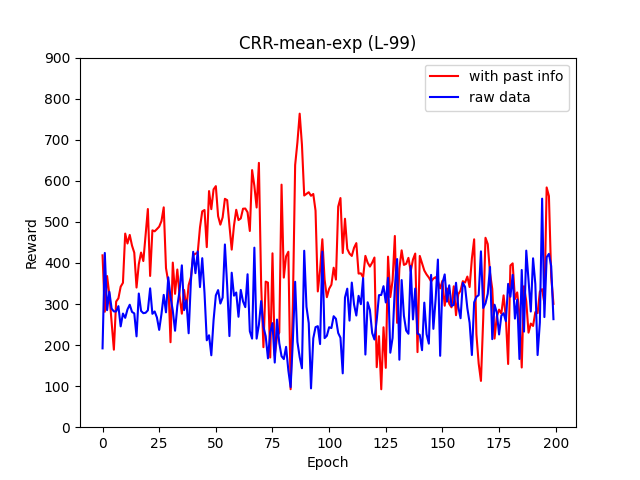
\includegraphics[width=3in]{CRR-mean-exp (L-99).png}
    \caption{CRR-mean-exp trained on ``finance-low-100".}
\end{minipage}
\end{figure}





\end{document}